\documentclass[a4paper,12pt,openany]{book}
\usepackage[T1]{fontenc}
\usepackage[utf8]{inputenc}
\usepackage{lmodern}
\usepackage{hyperref}
\usepackage{graphicx}
\usepackage{amsmath}
\graphicspath{ {images/} }
\usepackage[english]{babel}

%%%%%%%%%%%%%%%%%%%%%%%%%%%%%%%%%%%%%%%%%%%%%%%%
% Chapter quote at the start of chapter        %
% Source: http://tex.stackexchange.com/a/53380 %
%%%%%%%%%%%%%%%%%%%%%%%%%%%%%%%%%%%%%%%%%%%%%%%%
\makeatletter
\renewcommand{\@chapapp}{}% Not necessary...
\newenvironment{chapquote}[2][2em]
  {\setlength{\@tempdima}{#1}%
   \def\chapquote@author{#2}%
   \parshape 1 \@tempdima \dimexpr\textwidth-2\@tempdima\relax%
   \itshape}
  {\par\normalfont\hfill--\ \chapquote@author\hspace*{\@tempdima}\par\bigskip}
\makeatother


% Book's title and subtitle
\title{\Huge \textbf{Simulating Starlings Murmuration}}\\ 
% Author
\author{\textsc{Deepanshu Jindal} \\ \textsc{Arpan Mangal}}

\begin{document}

\frontmatter
\maketitle

\tableofcontents

\mainmatter

\chapter*{Preface}
This documents details the mathematical modelling and functional design for an application for simulating the flocking behaviour shown by Starlings: often known as Starlings murmuration.\\
\begin{figure}[h]
\centering
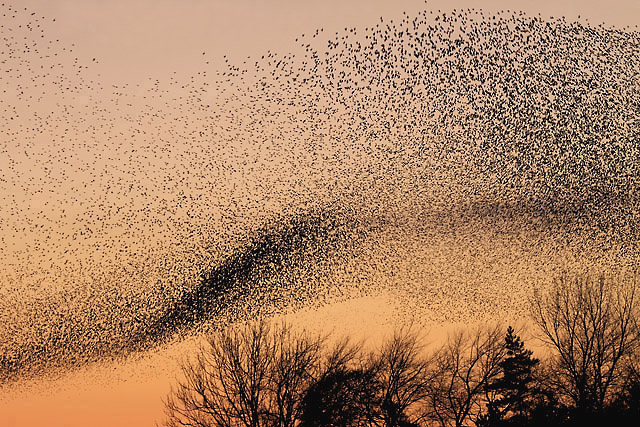
\includegraphics[scale=0.4]{Starling_murmuration.jpg}
\caption{Starlings murmuration}
\end{figure}
\\
Starlings murmuration is a type of swarm behaviour. From an abstract point of view, swarm behaviour is the collective motion of a large number of self-propelled entities. From the perspective of the mathematical modelling, it is an emergent behaviour arising from simple rules that are followed by individuals and does not involve any central coordination.\\

To model this we would use the boids program created by Craig Reynolds as an inspiration.
\\


\chapter{Mathematical Model}

\section{Intuition behind the model}
From the general observation of swarm behaviour we can identify some basic rules which we can assume that each member of the swarm is following:

1. Alignment : Move in the same direction as your neighbours

2. Cohesion : Remain close to your neighbours

3. Separation : Avoid collisions with your neighbours
\\
Apart from these basic rules, we can add in several assumptions such as they try to stay above a sleeping site, and when they happen to move outwards from the sleeping site, they return to it by turning. 


\section{Extension to the rules}
We bring in obstacle avoidance and wall avoidance properties so as to confine the boids to a certain section of the space.
\\
We add in random noise to the motion of each bird to bring in the effect of constant stirring motion.

\section{Assumptions}
\begin{enumerate}
	\item The birds fly with a fixed speed, lets call it $v_{max}$.
	\item The birds can change the direction vector of velocity by a fixed maximum amount say $\Delta v_{max}$.
	\item A bird's motion is influenced by its $n_{c}$ closest neighbours only.
	
\end{enumerate}

\section{Quantification of the rules}
We mathematically describe the computation for a particular bird. Let there be \emph{n} birds in the flock.\\
Let the velocities and position vectors of birds be represented by $\vec{v_1},\vec{v_2},\vec{v_3} ... \vec{v_n}$ and $\vec{r_1},\vec{r_2},\vec{r_3} ... \vec{r_n}$ respectively. \\

\noindent We define some predicates that would be useful for further computations

Let us define a predicate $p$ as

\begin{center}
\begin{equation}
	p(i,k) = 
\[ \begin{cases} 
      1 & \mid \vec{r_{ik}} \mid\ < \epsilon$\\
      0 & otherwise 
   \end{cases}
\]
\end{equation}
\end{center}	

Let us define a predicate $n$ as 
\begin{center}
\begin{equation}
	n(i,k) = 
\[ \begin{cases} 
      1 & bird\; i\; \epsilon\; the\; set\; of\; n_{c}\; closest\; neighbours\; of\; bird\; k\\
      0 & otherwise 
   \end{cases}
\]
\end{equation}
\end{center}	

\noindent Now, for $k^{th}$ bird,\\
First, we initialise $\vec{\Delta v_k} = 0$.\\


\\
\noindent Change in velocity due to rule of separation,
\begin{equation}
	\vec{\Delta v_k} += - \alpha \, p(i,k) \frac{\vec{r_{ik}} }{\mid \vec{r_{ik}} \mid ^2}
\end{equation}
where $\alpha$ is the hyper-parameter controlling separation.\\

\noindent Change in velocity due to rule of alignment,
\begin{equation}
	\vec{{av}_k} = \sum_{i=1}^{n} n(i,k)\vec{v_i}
\end{equation}
\begin{equation}
	\vec{\Delta v_k} += \beta \, \frac{\vec{{av}_{ik}} }{\mid \vec{{av}_{k}} \mid}
\end{equation}
where $\beta$ is the hyper-parameter controlling alignment.\\

\noindent Change in velocity due to rule of cohesion,
\begin{equation}
	\vec{{ar}_k} = \sum_{i=1}^{n} n(i,k)\vec{r_i}
\end{equation}
\begin{equation}
	\vec{\Delta v_k} += \gamma \, \frac{\vec{{ar}_{k}} - \vec{r_k} }{\mid \vec{{ar}_{k}} - \vec{r_k} \mid}
\end{equation}
where $\gamma$ is the hyper-parameter controlling cohesion.\\

\noindent Introduction of noise 
\begin{equation}
	\vec{\Delta v_k} += \delta \, \frac{random(\vec{a}) }{\mid random(\vec{a}) \mid}
\end{equation}
where $\delta$ is the hyper-parameter controlling noise.\\

\noindent Introduction of wall avoidance
We model our confinement area as a sphere of radius $R$ centred at origin
\begin{equation}
	\vec{\Delta v_k} += -\mu \, \frac{\vec{r_k}}{R - \mid \vec{r_k} \mid}
\end{equation}
where $\mu$ is the hyper-parameter controlling noise.\\

Subsequently, we bring into account the fact that maximum change in velocity is limited.\\
\begin{equation}
	scale = min(\Delta v_{max} , \mid \Delta \vec{v_k} \mid)
\end{equation}
We do this for all the birds and then in one pass update the direction vector for velocity for each bird.
\begin{equation}
	\vec{v_k} \,+=  scale \, \frac{\Delta \vec{v_k}}{\mid \Delta \vec{v_k}\mid}
\end{equation}

\noindent Finally, we update the position vectors for all the birds as
\begin{equation}
	\vec{r_k} \,+=  v_{max} \, \frac{\vec{v_k}}{\mid \vec{v_k}\mid}
\end{equation}

\chapter{Functional Specification}

The model will be developed as an application, consiting mainly of the flow shown below. 

\begin{figure}[h]
\centering
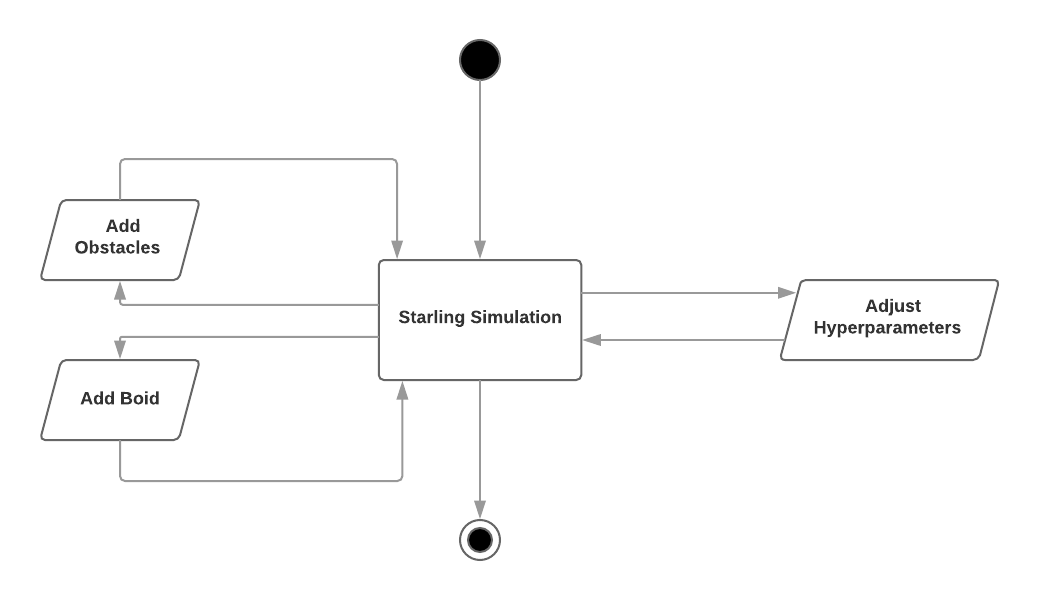
\includegraphics[scale=0.9]{UserFlowDiagram}
\caption{User Flow Diagram}
\end{figure}

The boids will be simulated in 3D, according to the mathematical model as described in the previous chapter. The simulation is based on the real flocking behaviour of Starlings. The user will be shown the various scientific results of the simulation.

\subsection*{Features}

The simulation starts with display of an initial number of boids. These are simulated according to some default value of hyper-parameters. There is a spherical wall enclosing the simulation space, which acts like confinement area for the boids.

The user can interact with the simulation in multiple ways:
\begin{itemize}

\item Add Boid(s) into the simulation with a mouse click
\item Tweak various hyper-parameters. These include:
\begin{itemize}
\item Separation Factor
\item Cohesion Factor
\item Alignment Factor
\item Noise Factor
\item Speed of boids
\item Maximum acceleration that the boids can produce
\end{itemize} 

\item Rotate the simulation view to be able to see the simulation from various angles.

\end{itemize}

\subsection*{Measurements}
The user will be constantly be shown the following results. He / she can tweak the hyper-parameters to see how the simulation will appear and see the corresponding changes in the result values.
\begin{itemize}
\item \textbf{Power}: The power being consumed by an average bird as well as the power consumed by the complete flock at the particular instant of time.
\item \textbf{Acceleration}: The average magnitude of acceleration being produced by each bird.
\item \textbf{Energy}: The total energy consumed by an average bird from the start of the simulation.
\item \textbf{Angular Momentum}: The average magnitude of angular momentum of a typical bird.
\end{itemize}

\end{document}
